%%%%%%%%%%%%%%%%%%%%%%%%%%%%%%%%%%%%%%%%%
% Journal Article
% LaTeX Template
% Version 1.4 (15/5/16)
%
% This template has been downloaded from:
% http://www.LaTeXTemplates.com
%
% Original author:
% Frits Wenneker (http://www.howtotex.com) with extensive modifications by
% Vel (vel@LaTeXTemplates.com)
%
% License:
% CC BY-NC-SA 3.0 (http://creativecommons.org/licenses/by-nc-sa/3.0/)
%
%%%%%%%%%%%%%%%%%%%%%%%%%%%%%%%%%%%%%%%%%

%----------------------------------------------------------------------------------------
%	PACKAGES AND OTHER DOCUMENT CONFIGURATIONS
%----------------------------------------------------------------------------------------

\documentclass[twoside,twocolumn]{article}
\usepackage{graphicx} % For tables and graphs
\usepackage{amsmath, amsthm, amssymb} % for equations
\usepackage{hhline} % For double lines in Table
\usepackage{nicefrac} %For inline fractions

\usepackage{blindtext} % Package to generate dummy text throughout this template 

\usepackage[sc]{mathpazo} % Use the Palatino font
\usepackage[T1]{fontenc} % Use 8-bit encoding that has 256 glyphs
\linespread{1.05} % Line spacing - Palatino needs more space between lines
\usepackage{microtype} % Slightly tweak font spacing for aesthetics

\usepackage[english]{babel} % Language hyphenation and typographical rules

\usepackage[hmarginratio=1:1,top=32mm,columnsep=20pt,margin=1in]{geometry} % Document margins
\usepackage[hang, small,labelfont=bf,up,textfont=it,up]{caption} % Custom captions under/above floats in tables or figures
\usepackage{booktabs} % Horizontal rules in tables

\usepackage{lettrine} % The lettrine is the first enlarged letter at the beginning of the text

\usepackage{enumitem} % Customized lists
\setlist[itemize]{noitemsep} % Make itemize lists more compact

\usepackage{abstract} % Allows abstract customization
\renewcommand{\abstractnamefont}{\normalfont\bfseries} % Set the "Abstract" text to bold
\renewcommand{\abstracttextfont}{\normalfont\small\itshape} % Set the abstract itself to small italic text

\usepackage{titlesec} % Allows customization of titles
\renewcommand\thesection{\Roman{section}} % Roman numerals for the sections
\renewcommand\thesubsection{\arabic{section}.\arabic{subsection}} % Lower Case Roman numerals for subsections subsections
\titleformat{\section}[block]{\large\scshape\centering}{\thesection}{1em}{} % Change the look of the section titles
\titleformat{\subsection}[block]{\large}{\thesubsection}{1em}{} % Change the look of the section titles
\titleformat{\subsubsection}[block]{\large\bfseries}{}{1em}{} % Change the look of the section titles

\usepackage{fancyhdr} % Headers and footers
\pagestyle{fancy} % All pages have headers and footers
\fancyhead{} % Blank out the default header
\fancyfoot{} % Blank out the default footer
\fancyhead[C]{Ring Identification Algorithm --- August 2016 --- IPP Summer Student 2016} % Custom header text
\fancyfoot[RO,LE]{\thepage} % Custom footer text


\usepackage{titling} % Customizing the title section

\usepackage{hyperref} % For hyperlinks in the PDF

%----------------------------------------------------------------------------------------
%	TITLE SECTION
%----------------------------------------------------------------------------------------

\setlength{\droptitle}{-4\baselineskip} % Move the title up

\pretitle{\begin{center}\Huge\bfseries} % Article title formatting
\posttitle{\end{center}} % Article title closing formatting
\title{Particle Identification in Cherenkov Detectors using Convolutional Neural Networks} % Article title
\author{%
\textsc{Theodore Tomalty} \\[1ex] % Your name
\normalsize \href{mailto:theo@tomalty.com}{theo@tomalty.com}\\~\\ % Your email address
\normalsize University of Toronto \\ % Your institution
\normalsize Institute for Particle Physics \\
%\and % Uncomment if 2 authors are required, duplicate these 4 lines if more
%\textsc{Jane Smith}\thanks{Corresponding author} \\[1ex] % Second author's name
%\normalsize University of Utah \\ % Second author's institution
%\normalsize \href{mailto:jane@smith.com}{jane@smith.com} % Second author's email address
}
\date{\today} % Leave empty to omit a date
\renewcommand{\maketitlehookd}{%
\begin{abstract}
\noindent Cherenkov Detectors measure light radiated in a cone by charged particles moving faster than light in a medium. They emulate a camera with its pixels facing inwards around the detection chamber. For the problem of particle identification in these detectors, visual signatures in the emitted radiation are analyzed. For example, the standard analysis of the Super-Kamiokande detector in Japan is complete with likelihood fits for $e$-$\mu$ separation. In this project we will explore the use of machine learning methods, particularly convolutional neural networks, in order to outperform the standard analysis in $e$-$\mu$ separation for Super-K.
\end{abstract}
}

%----------------------------------------------------------------------------------------

\begin{document}


% Print the title
\maketitle
\thispagestyle{fancy}

%----------------------------------------------------------------------------------------
%	ARTICLE CONTENTS
%----------------------------------------------------------------------------------------

\section{Introduction}

\lettrine[nindent=0em,lines=3]{C}{herenkov} detectors are used for charged particle identification. When a charged particle moves through a medium faster than light can propagate in that medium, Cherenkov radiation is released in the shape of a cone in the direction of movement. The interior of the Cherenkov detector is instrumented with PMTs to detect this Cherenkov light. Particles, then, can be identified by the shapes of the images on the detector walls.

In neutrino experiments, water Cherenkov detectors are commonly used to distinguish between electrons and muons, which determines the flavour of the interacting neutrino in the medium. An example of this kind of detector is Super-Kamiokande  \cite{cite:SuperK}: a cylinder filled with 50 kilotonnes of water located underground in Japan.

Standard event identification uses likelihood fits to the PMT charge and timing information. In particular, theoretical Cherenkov cones are fitted to the raw data using different particle-type hypotheses, to see which one corresponds best. This project will test the use of a machine learning algorithm as an alternative to the standard $e$-$\mu$ separation, and compare its performance to the methods already in practice.

Specifically, we will be using a Python machine learning framework, Tensorflow \cite{cite:tensorflow}, to train a Convolutional Neural Network (CNN). The goal will be to achieve the highest classification performance possible on simulated electron and muon events in Super-K.

\subsection{Cherenkov Radiation}

A Cherenkov detector measures any light that is produced in its dark cavity where the light mostly comes from Cherenkov radiation of charged particles, analogous to a sonic boom when an aircraft breaks the sound barrier.

A charged particle that moves in a medium will emit concentric wavefronts of electromagnetic radiation as in figure \ref{fig:ConeFront}. When the particle moves faster than $\frac{c}{n}$, the wavefronts interfere constructively with each other in a conical trajectory through the medium.

\begin{figure}[ht]
    \centering
    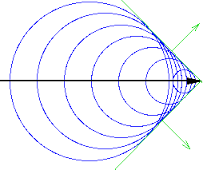
\includegraphics[width=0.38\textwidth]{ConeFront.png}
    \caption{Diagram depicting the wavefront of Cherenkov radiation of a charged particle moving faster than light in a medium.}
    \label{fig:ConeFront}
\end{figure}

Charged particles in a Cherenkov Detector originate at random positions in the detector volume, ideally from interactions between the water and passing neutrinos. The vertex of these particles will correspond to the centre of the largest circle in figure \ref{fig:ConeFront} and, as such, the Cherenkov radiation will propagate outwards at a fixed angle with respect to that vertex position. The result is a conical projection of light onto the detector walls, like a flashlight shining from the particle vertex.

Cherenkov radiation manifests on the detector wall in the shape of rings. These are measured by the PMTs to produce an event display similar to figures \ref{fig:ElectronRing} or \ref{fig:MuonRing}. The shape of the Cherenkov rings depend on the type of particle that generated them, and so the shape can be used to identify the particle.

\begin{figure}[ht]
    \centering
    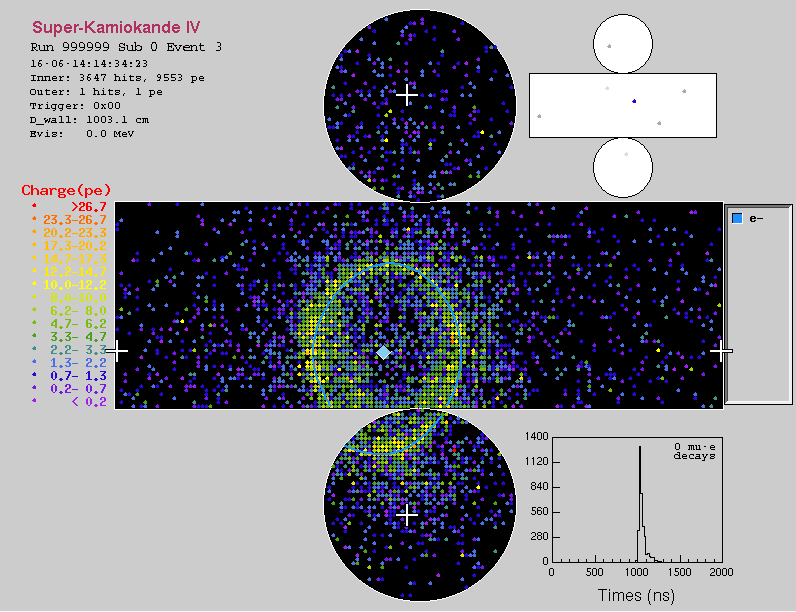
\includegraphics[width=0.3\textwidth]{ElectronRing.png}
    \caption{Display of the PMT readout of Super-K detector in the case of a single electron.}
    \label{fig:ElectronRing}
\end{figure}

\begin{figure}[ht]
    \centering
    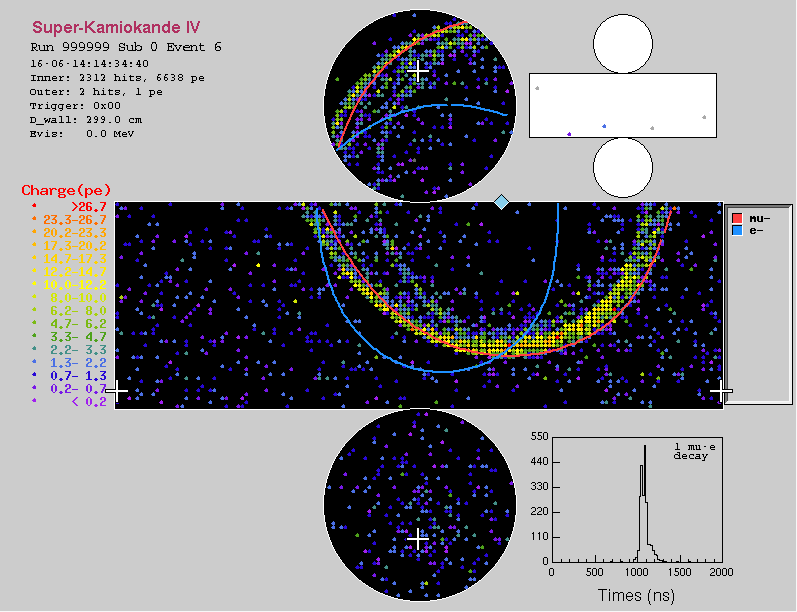
\includegraphics[width=0.3\textwidth]{MuonRing.png}
    \caption{Display of the PMT readout of Super-K detector in the case of a single muon.}
    \label{fig:MuonRing}
\end{figure}

As mentioned in the introduction, we will be focusing on the identification of electron and muon rings. By comparing the electron ring in figure \ref{fig:ElectronRing} with the muon ring in figure \ref{fig:MuonRing} one can see that electrons produce much fuzzier rings than muons do. This is a result of electron trajectories being much more scattered than those of muons, and will be the key feature to exploit in particle identification.

Given a set of initial parameters (such as position of interaction, direction and energy of particle, type of particle, etc.) the distribution of light on the detector walls can be predicted by mapping the theoretical emission profile onto the cylinder. In this way, the standard fiTQun algorithm varies each continuous variable to minimize the difference between predicted and observed PMT output for each assumed particle type. When the maximum likelihood is found in the parameter space of each type, the particle is identified by comparing the likelihood of the particle types with each other, and selects the maximum.

\subsection{Machine Learning}

Machine learning methods are used in this project because they are robust in the presence of statistical variation from case to case. They learn features automatically without the need for as much tuning as likelihood fits. Since this is a visual problem we will attempt to emulate human classification by implementing a specific type of neural network that is based on mammal vision.

\subsubsection{Simple Network}

The principles of machine learning are in fact quite simple. The standard problem is to have a set of objects, which can be images, soundbites, or just lists of numbers, and a set of possible classifications for those objects. Given a random set of objects, the job is to classify them based on their numerical input parameters (pixel intensity, Fourier decomposition, etc.) 

The simplest network assigns weights between each input parameter and each possible classification. If one input channel is correlated with a specific classification, the network will consider a presence of that input as evidence towards the corresponding classification. Suppose that you collect all the inputs into a vector $x_i$ of size $N$, and there are $P$ possible classifications. The output of the network will be an evidence$_j$ vector of size $P$, with one channel for each classification.

The variable weights, described above, for each input-output pair are collected into a matrix $M_{ji}$. Evidence for each classification is then a matrix multiplication, given by equation \ref{eqn:evidence}, where we have added a $b_j$ vector to represent a statistical bias in the set of objects to account for some classifications being more likely than others.

\begin{equation}\label{eqn:evidence}
    \text{evidence}_j = \sum_{i=1}^{N}M_{ji}x_{i} + b_j
\end{equation}

The network submits as a prediction whichever classification accumulates the most evidence in its favour. In fact, one can evaluate the confidence of the network for each classification by performing a softmax transformation of the evidence using equation \ref{eqn:softmax}.

\begin{equation}\label{eqn:softmax}
    p_j = \frac{\exp(\text{evidence}_j)}{\sum_j\exp(\text{evidence}_j)}
\end{equation}

The values of $M_{ji}$ and $b_j$ are not known \textit{a priori}. They must be optimized for a particular problem during a training process. To do this we define a continuous function that quantifies the imperfection of the network, called the network loss (or cost function), and minimize it on a set of training objects.

The simple cost function in equation \ref{eqn:loss} is defined by the $L^2$ norm distance between the network prediction and the ideal output. Equation \ref{eqn:softmax} is used to represent the network prediction because the terms sum to unity, and the ideal case is set to a $q_i$ vector of the form $[0, 0, 1, 0, ...]$ with 1 in the true classification channel.

\begin{equation}\label{eqn:loss}
    D = \sum_{\text{images}} |{\bf{p}} - {\bf{q}}|^2
\end{equation}

Training the network then becomes as simple as minimizing the loss function in the space of parameters $M_{ji}$ and $b_i$. Assuming that this type of classification is appropriate for the task at hand, optimizing these parameters on a large training set of objects should enable the network to classify well an independent set of test objects.

For more complicated problems it is common to implement hidden layers of neurons in the network (see figure \ref{fig:SimpleNet}). We use the same linear transformation as in equation \ref{eqn:evidence} except instead of using weights that map directly to the evidence, we map to an arbitrary number of \textit{neurons} and then map those neurons to the output predictions (one set of matrix weights and biases for each map, and apply softmax only at the very end).

In this way, each neuron can be activated for a particular configuration of the input. The network is then able to learn \textit{features} of the input, considering multiple channels, rather than just single input-output correlation. Depending on the problem there can be as many hidden layers, and as many neurons, as you want. But adding complexity to the network when the problem does not warrant it usually causes problems due to overfitting and irregularities in the loss function topology.

\begin{figure}
    \centering
    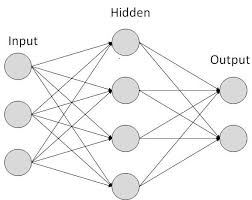
\includegraphics[width=0.38\textwidth]{SimpleNet.jpeg}
    \caption{Simple neural network with one hidden layer of 4 neurons.}
    \label{fig:SimpleNet}
\end{figure}

\subsubsection{Convolutional Neural Networks}

The networks described in the previous section work well when data can be characterized with numerical values, and each value or combination of values is associated with specific classifications. In image recognition the set of pixel intensities are used as input. A simple network, then, would map each pixel to the hidden layers and then to the output classification. Each neuron could be activated by a certain combination of inputs, and so to recognize a face, for example, the network would have to have one neuron dedicated to each possible face position, angle, shading, scale, etc.

This is, of course, impossible because the combinations are too great, and so an alternative method must be introduced. Just as the simple network reflects logic processing in a human brain, mammal vision will be the template for an image recognition network. Rather than forming connections associated with every possible view, our brains scan the field of vision for specific features, organizes those features into shapes, and combines those shapes into objects.

\begin{figure}[ht]
    \centering
    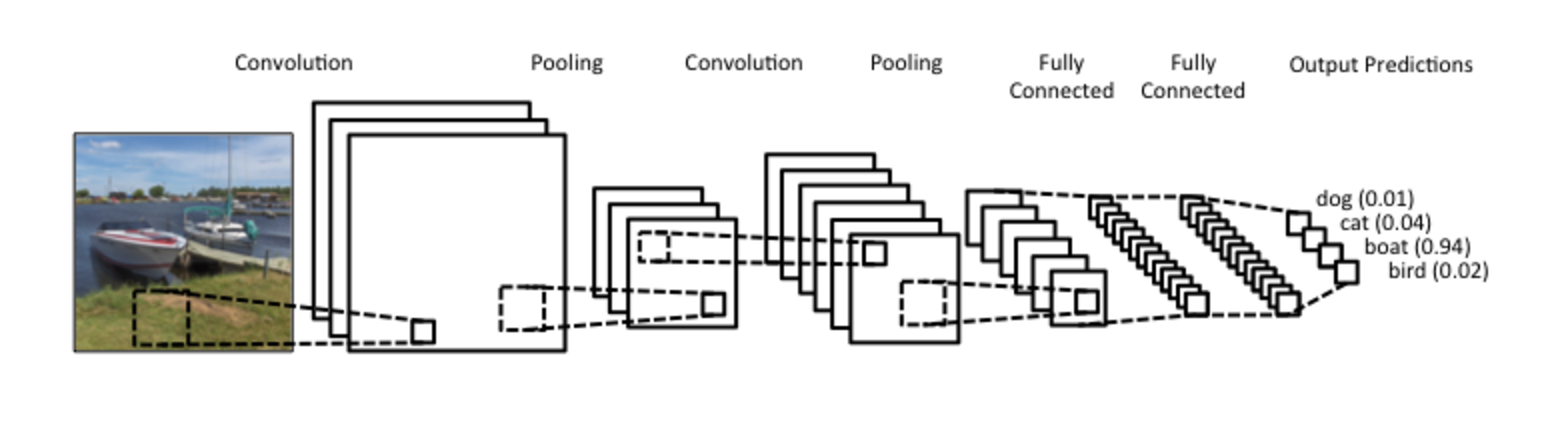
\includegraphics[width=0.45\textwidth]{CNN.png}
    \caption{Diagram of a Convolutional Neural Network (CNN) used for classifying images.}
    \label{fig:CNN}
\end{figure}

A Convolutional Neural Network (CNN) follows the same principles. Rather than classifying an image based on its complete pixel input, the network makes use of a set of $J$ filters, each one a square of weight variables (like a small $n\times n$ image), that corresponds with a particular feature on the image. The filters are scanned across the original image, in a discrete convolution, to produce feature maps that are activated in regions where the corresponding filter is in accordance with the image.

Typically, filters for the first convolution represent generic features like an edge, a colour gradient, or a texture. In order to classify more complex objects a second convolution is performed, this time with filters that have an independent set of weights for each feature map. That way it is able to identify combinations of activated features in a region that, when grouped, correspond to a shape. A third convolution can be performed to group combinations of shapes into objects.

After each convolution it is standard to down sample the maps by pooling the pixels together. This is done because each level of complexity requires less resolution. It is usually more important that a feature exists in a certain region than the exact topology of that feature on the feature map, and it is always beneficial to reduce the number of weights that need to be optimized when possible.

At the end of this process we are left with many feature maps that indicate which objects are present in the image and, roughly, where those objects are in relation to each other. All that is left to do is to pass this information into a standard neural network, complete with hidden layers of neurons, to classify the image. For example, in facial recognition, the output objects of the convolution layer might be blue eyes, thin nose, wide ears, etc. and the classification would be the person's name whose face it is.

\section{Data and Processing}

To train a neural network, a large number of of statistics are required. The standard Super-K particle simulation was run on 400,000 events that were split into a training sample and a testing sample. An equal number of electrons and muons are generated, with vertexes homogeneously distributed in the detector volume and initial energy evenly distributed between 300MeV and 1GeV. Each event in the simulation returns a map of the detector response including PMT integrated charge, which is proportional to light intensity, and timing information. The standard analysis fitting algorithm, fiTQun \cite{cite:fiTQun_poster} \cite{cite:fiTQun}, is run on all of these events to return a particle-type prediction as well as approximations of the particle's kinematics (e.g. vertex position and momentum).

\subsection{Image Production}

Each PMT in a Cherenkov detector produces a measure of light intensity and has a fixed position in 3D space, much like a single pixel on a cylindrical image. Convolutional Neural Networks function by scanning square images, using different filters, to identify features. A first problem we encounter is that of generalizing flat convolution (scanning) to a cylindrical one. Another problem arises because particles can originate at any point in the detector, and move in any direction, so there are many degrees of freedom in the shape of the rings on the cylinder. They can have different sizes, elongations, and further irregularities arising in the corners of the cylinder. Such ring deformations can make learning very difficult for the algorithm.

In order to simplify the problem we focus the algorithm on the Cherenkov profiles rather than their projection onto the cylinder. This is done, as indicated in figure \ref{fig:Cartoon}, using a conical projection of PMT charges onto a flat, transverse plane. The standard analysis reconstructed vertex is used as the point of origin for the projection. Instead of warped rings on a cylinder we will get circular rings on a flat image, so both problems described above are solved this way.

\begin{figure}[ht]
    \centering
    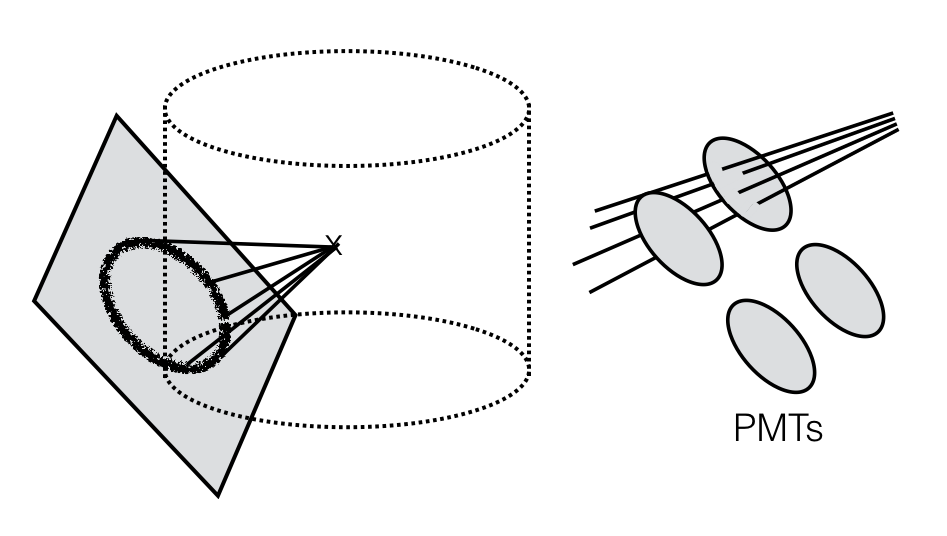
\includegraphics[width=0.45\textwidth]{Cartoon.png}
    \caption{Process the detector output by performing a conical projection of the PMT signals onto transverse-planar image.}
    \label{fig:Cartoon}
\end{figure}

A blank $30\times 30$ pixel image is set up in 3D space. It is centred at the intersection of the particle trajectory with the detector walls, normal to the direction of the particle, and its width and height are scaled with the distance traversed by the particle. The position of the plane is chosen so that the projected rings are centred, and so the resolution of the image can be compared to the resolution of the detector. The orientation of the image is chosen in order to ensure the rings are all circular. In addition, the image size is scaled to have a length and width proportional to the expected ring radius (so that all the rings appear the same size in the images).

Ring projections are done by considering the lines between each PMT and the particle vertex. If the line intersects the image, the corresponding PMT signal is added to the weight of the intersection pixel. This converts a complex shape on the detector wall to a circle on the image plane. It is often the case, however, that some PMTs are much closer to the vertex than others, and the resulting difference in angular resolution of the detector is enough to make the output image quite irregular. To smooth out the image, a flux of randomly distributed lines intersecting a PMT, as shown in figure \ref{fig:Cartoon}, are set to carry a fraction of the PMT's signal. These lines are projected onto the image individually instead of a single line projection per PMT.

The question of scaling was mentioned briefly above. The image size is set proportional to vertex-to-wall distance in the direction the particle travels. This way, since Cherenkov cones all have the same angle with respect to the vertex, the rings have the same radius on the output image. However, since it is not ideal to use an image resolution that is much higher than the PMT resolution, the events are separated into four image sets with different distance-to-wall ranges. Three of those sets are shown in figure \ref{fig:ProcessedRings}. Each set has a different size of ring on the image, selected to correspond with PMT resolution, but all the images in a single set have the same ring size. This way, we train a separate CNN for each set so that an individual network does not have to deal with differences in ring shape due to resolution issues.

\begin{figure}[ht]
    \centering
    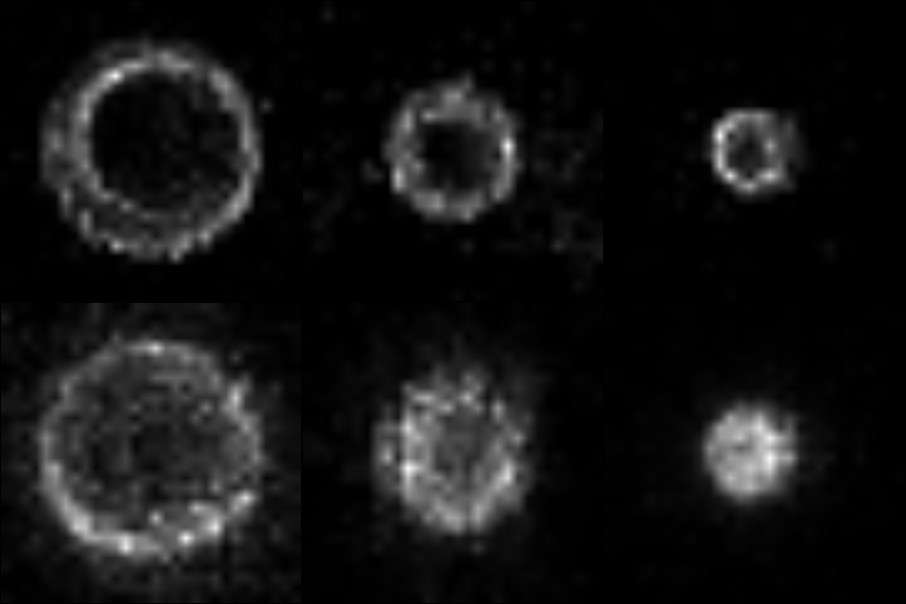
\includegraphics[width=0.45\textwidth]{ProcessedRings.png}
    \caption{Output images of the cone projection described in figure \ref{fig:Cartoon}. Top: muon rings, Bottom: electron rings, Left to Right: data set 1, 3, and 4.}
    \label{fig:ProcessedRings}
\end{figure}

\begin{itemize}
    \item[Set 1:]{
        These images scale the rings to take up most of the image. The lower bound on the distance-to-wall is selected so that the resolution of the detector is greater than that of the $30\times 30$ pixel image (evaluated at the centre of the image).
    }
    \item[Set 2:]{
        These rings are scaled to the same size as set 1 but here the distance between PMTs is larger than the size of the image pixels. In other words the resolution in these images is inflated artificially, and is done so until the algorithm performance was observed to fall off.
    }
    \item[Set 3:]{
        In this distance-to-wall range, the artificial resolution becomes a problem for the algorithm, and so the image size is set so that the pixels are, on average, 1.25 larger than PMT distances. The small scale factor is used in consideration of the fixed $5\times 5$ filter size shared between data sets.
    }
    \item[Set 4:]{
        These images follow the same logic as the previous set, except with particles that are closer to the detector walls so the rings are smaller on the images.
    }
\end{itemize}

Once this procedure returns a stream of square images of circular rings, like those in figure \ref{fig:ProcessedRings}, a cut must be made before passing these to the CNN. It is standard to remove events from the analysis with vertexes closer than 2m from the detector walls, so this cut is performed using the reconstructed vertex from fiTQun. In cases of particles very close the walls, however, the 2m cut can be insufficient because fiTQun greatly fails the vertex reconstruction due to lack of information. To remove the events that slipped through the first cut, seen in the left corner of figure \ref{fig:cut_leakage}, a second cut is done on events with less than 160 PMTs hit in the detector. 

\begin{figure}[ht]
    \centering
    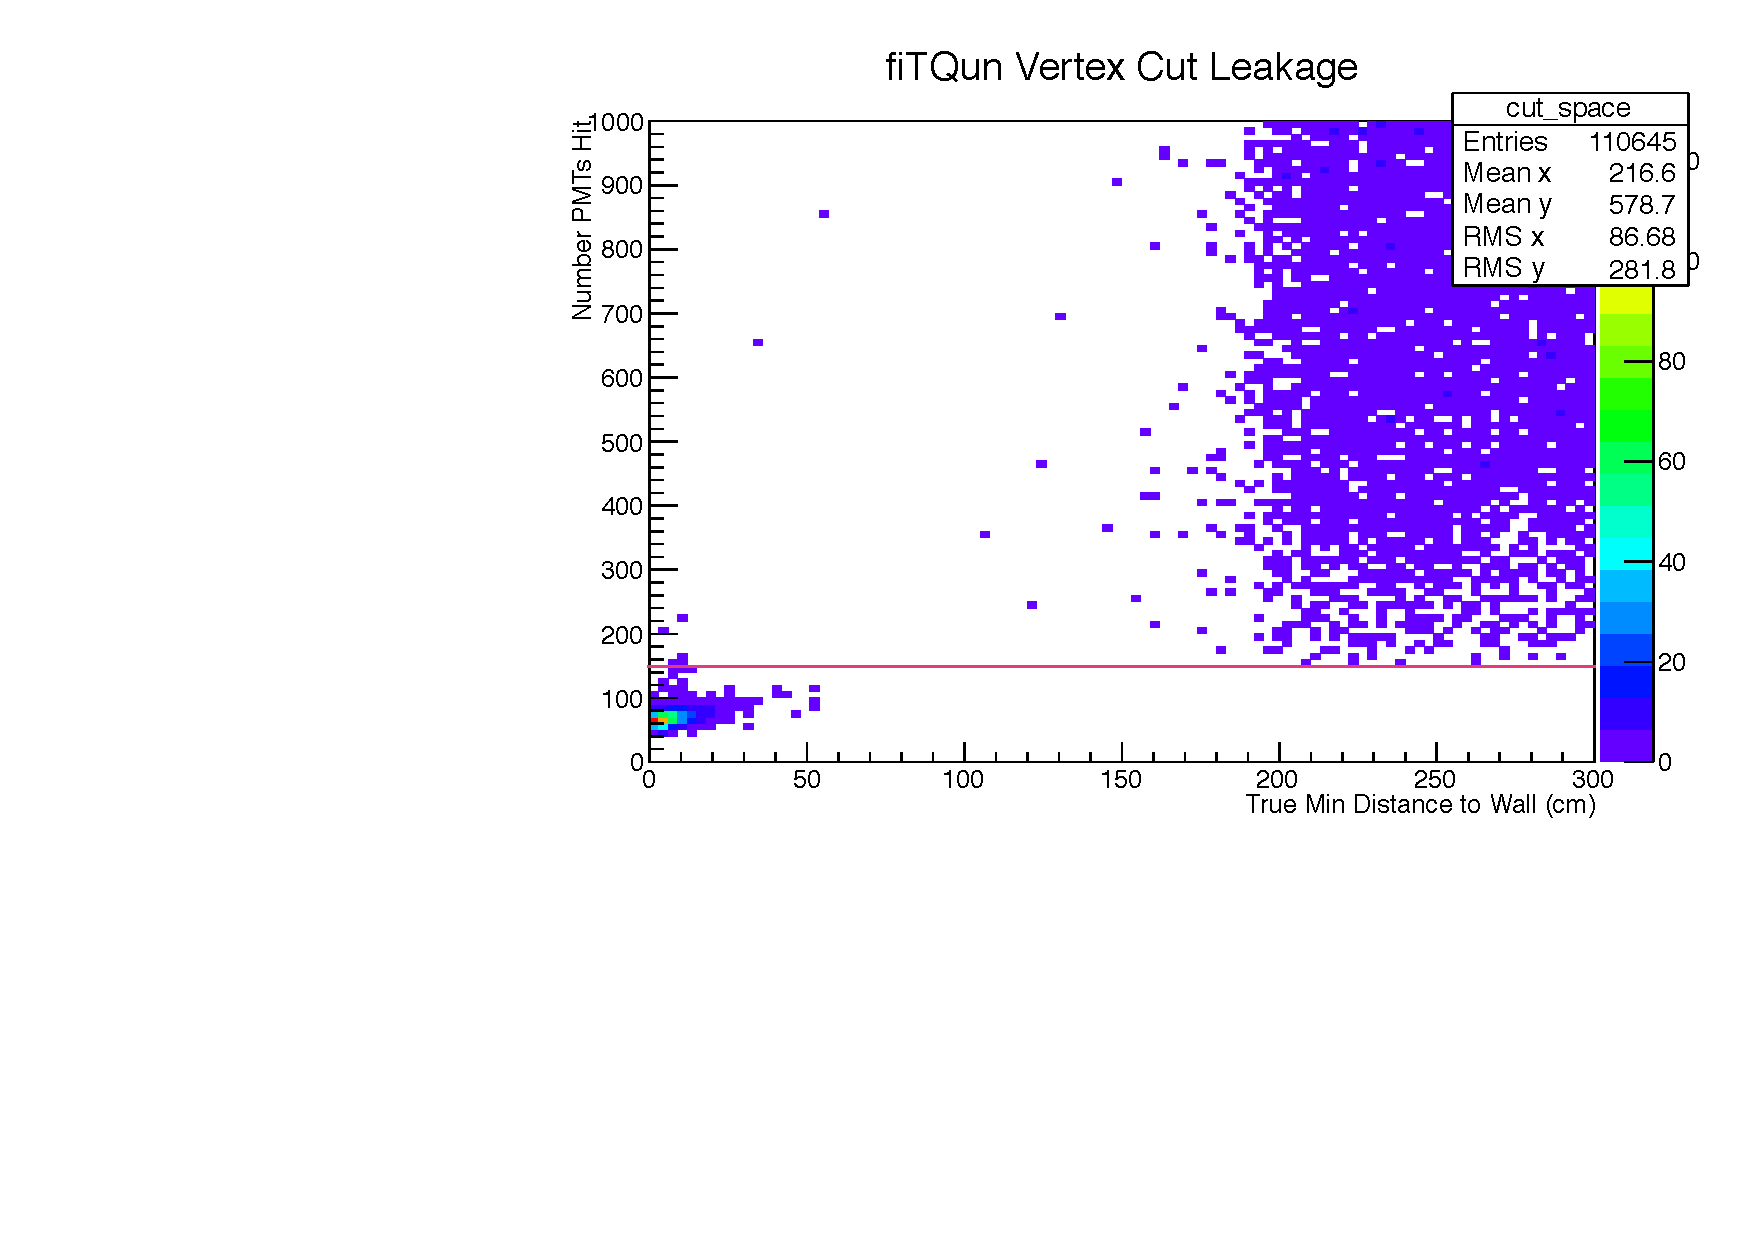
\includegraphics[width=0.45\textwidth]{cut_leakage.pdf}
    \caption{True distances of particles to the wall vs. the number of PMTs that registered hits with light. These events have already passed the fiTQun 2m-from-wall selection.}
    \label{fig:cut_leakage}
\end{figure}

\section{The Algorithm}

Convolutional neural networks \cite{cite:CNN} are standard for image recognition problems, and are used for this project. The algorithm takes input from $30\times 30$ pixel images, as in figure \ref{fig:ProcessedRings}, and will be tasked with classifying the rings as electron- or muon-shaped. The CNN will be designed to process images analogous to how a human might, that is by identifying sharp edges with muons and and fuzzy edges with electrons.

\subsection{Network Architecture}

For our network, $5\times 5$ pixel filters were used to correspond roughly with pixel scale of the ring edges. The filters were set manually in this project because the network was observed to have difficulty optimizing the filter shapes independently. The initial filters shown in figure \ref{fig:Initial} contain sharp and smooth edges, each rotated eight times for complete investigation of the circle, as well as reflection-invariant filters that will be used to probe the ring shape in general. 

\begin{figure}[ht]
    \centering
    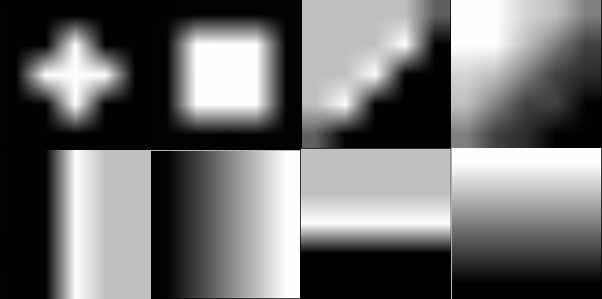
\includegraphics[width=0.45\textwidth]{Initial.png}
    \caption{Sample of the initial filters used in the convolution layer of the network. 22 filters total including 16 from smooth-sharp edges each rotated eight times.}
    \label{fig:Initial}
\end{figure}

The feature maps associated with each filter are pooled into $10\times 10$ images (using the maximum of each $3\times 3$ area from the feature map) and the pixels of the pooled images are linked directly into the classification network. In more complex image recognition problems a second convolution might be performed but our network does not need to perform high-level analysis of shapes aside from simple feature identification.

The classification network, then, consists of two neuron layers (with fourteen neurons each) before the two-channel output prediction as either muon or electron. This is a standard neural network with the purpose of converting visual information from the feature maps into a ring classification. Certain features, such as a smooth edge, can be weighted more or less strongly depending on where they occur, and the presence of two layers offers more complex logic in the classification if needed.

\subsection{Network Training}

With a large training set of images it is virtually impossible to minimize the network loss on all the data at once, so each step in the minimizing procedure uses a random batch of 200 images. Step size must be chosen carefully to not overstep global topology while also not getting stuck in local fluctuations. Simple trial and error of different step sizes is done until training successfully begins reducing the average losses. Recall that there are four separate CNNs, that operate on individual image sets. Each network is trained in parallel on independent batches of images.

This stochastic method works well in learning general features that are shared between many images, but easily \textit{forgets} important features that appear rarely. For that reason, the network parameters are saved in an averaged quantity that contains components from all previous steps (older steps are weighted less). The decay rate is selected so that roughly 500 of the latest steps are significant in the average, which corresponds to 100,000 images, so that most images in the training sample will be represented by the network. Testing is done on the averaged parameters rather than the parameters in the most recent step. As the algorithm converges, the step size is also reduced exponentially so that the parameters can settle in a true local minimum.

The training process provides a second reason to split the images up into different sets. Each set contains rings that look similar to each other, but that are significantly different when compared between sets. Roughly 80\% of the images are in set 1, 10\% in set 2, and 5\% in both 3 and 4. So if the networks are trained on the same batch, images of type 2, 3, and 4 have effective batch sizes that are problematically small. Therefore, for the training process, the images in each set are separated into individual directories, and each of the four networks are trained in parallel using batches saturated with their own image types. 

\section{Results}

The total accuracy of the CNN is shown in figure \ref{fig:algorithm_vs_2s}. But, for context, it is useful to compare the performance of the CNN to the standard analysis (fiTQun) in the case of single ring $e$-$\mu$ separation. It is first necessary evaluate the performance of fiTQun.

\subsection{Standard Analysis}

FiTQun fits theoretical Cherenkov cones to the PMT time and charge information using different particle hypotheses. The Cherenkov cone with the largest maximum likelihood is selected to represent the event, providing a reconstructed particle type, vertex position, energy, etc.

The simplest fiTQun configuration, to compare with the CNN, uses two single ring fits: one electron fit and one muon fit. The accuracy of this regime is plotted in figure \ref{fig:fiTQun_v_ms} in red. As expected, events in the second, third, and fourth image sets perform subsequently worse because the rings are smaller. There is, however, a significant dip in the performance for muons in the first image set. Investigation reveals that this region is populated by images with more than one ring, most likely from muons that have a segmented trajectory due to scattering.

\begin{figure}[ht]
    \centering
    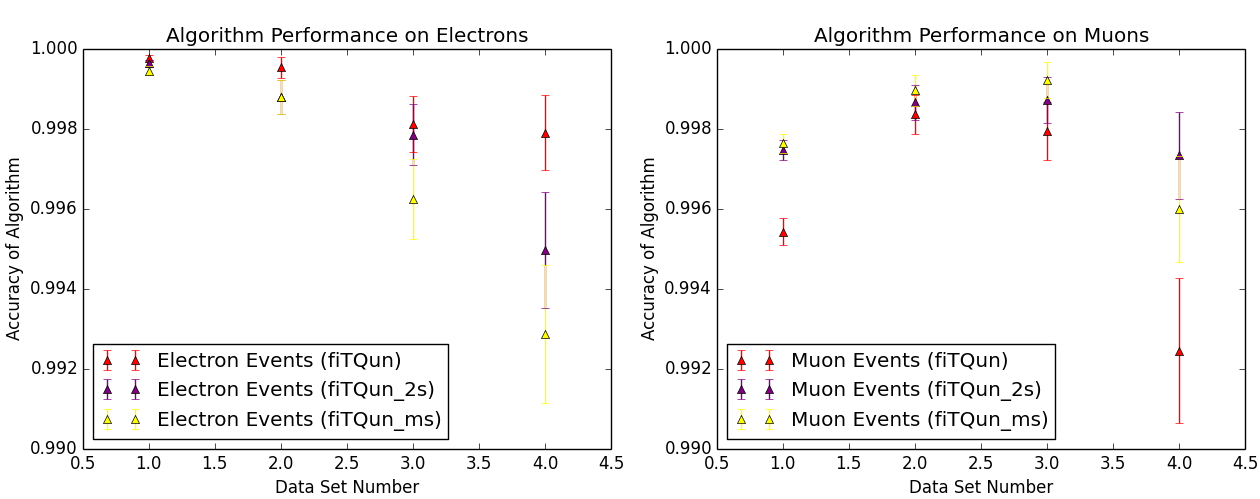
\includegraphics[width=0.48\textwidth]{fiTQun_v_ms.png}
    \caption{Performance of three fiTQun regimes for electron and muon events and each image set. Red: default fiTQun with single ring electron and muon fits (99.77\%), Purple: fiTQun with two-ring segmented muon fit (99.846\%), Yellow: fiTQun with three-ring segmented muon fit (99.836\%).}
    \label{fig:fiTQun_v_ms}
\end{figure}

To improve the identification performance on these cases, an augmented muon fit strategy is used that searches for secondary rings. The algorithm performances using two- and three-ring searches are plotted in figure \ref{fig:fiTQun_v_ms} in purple and yellow respectively. It can be observed that the two-ring segmented regime represents the best total classification performance of the standard analysis.

\subsection{Performance Comparison}

Once the CNN is trained on two training runs of 1500 batches, the results are plotted in figure \ref{fig:algorithm_vs_2s} with the best fiTQun regime for comparison. The two algorithms are similar in performance except in the first and last muon bins. There are far more events in the first bin, however, so in total the CNN recovers roughly 30\% of the standard analysis classification performance. In reality, however, the CNN structure is most comparable to a regime of fiTQun that does not use timing information and which is not tuned for segmented rings. In that case it recovers close to 70\% of the performance.

\begin{figure}[h]
    \centering
    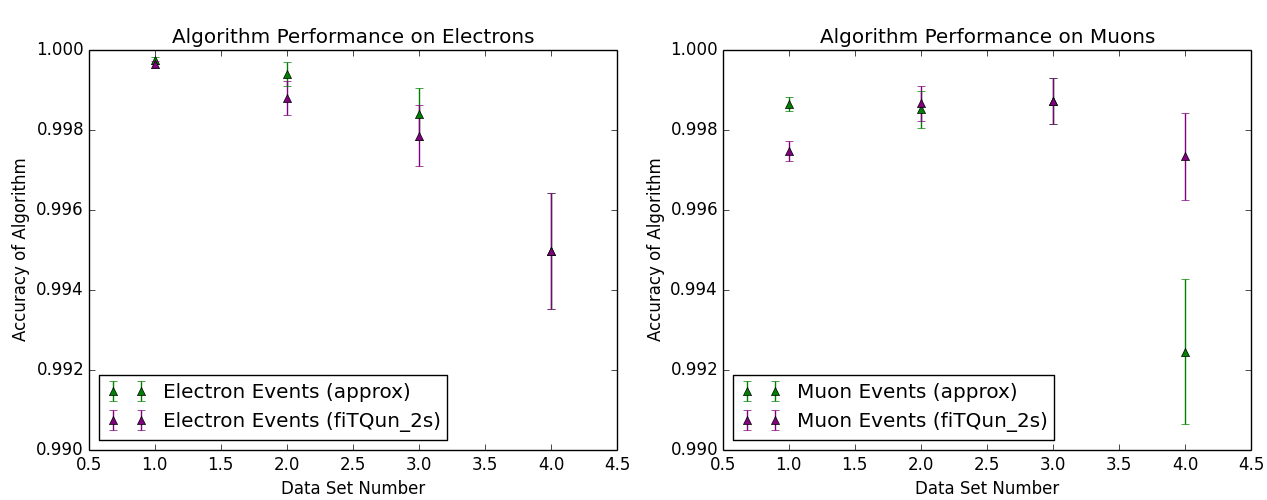
\includegraphics[width=0.48\textwidth]{algorithm_vs_2s.png}
    \caption{Comparison of CNN classification (Green: 99.89\%) to fiTQun with two-ring segmented muon fit (Purple: 99.846\%).}
    \label{fig:algorithm_vs_2s}
\end{figure}

In order to better compare these two classification algorithms, we can plot the events in a 2D histogram with the softmax output of the CNN in one axis and the negative log likelihood measure from fiTQun in the other (see fig. \ref{fig:Phase_Space_Approx}). The lower left-hand plot is of particular interest because set-1 muons contribute the most to the problematic events in both classification methods.

\begin{figure}[h]
    \centering
    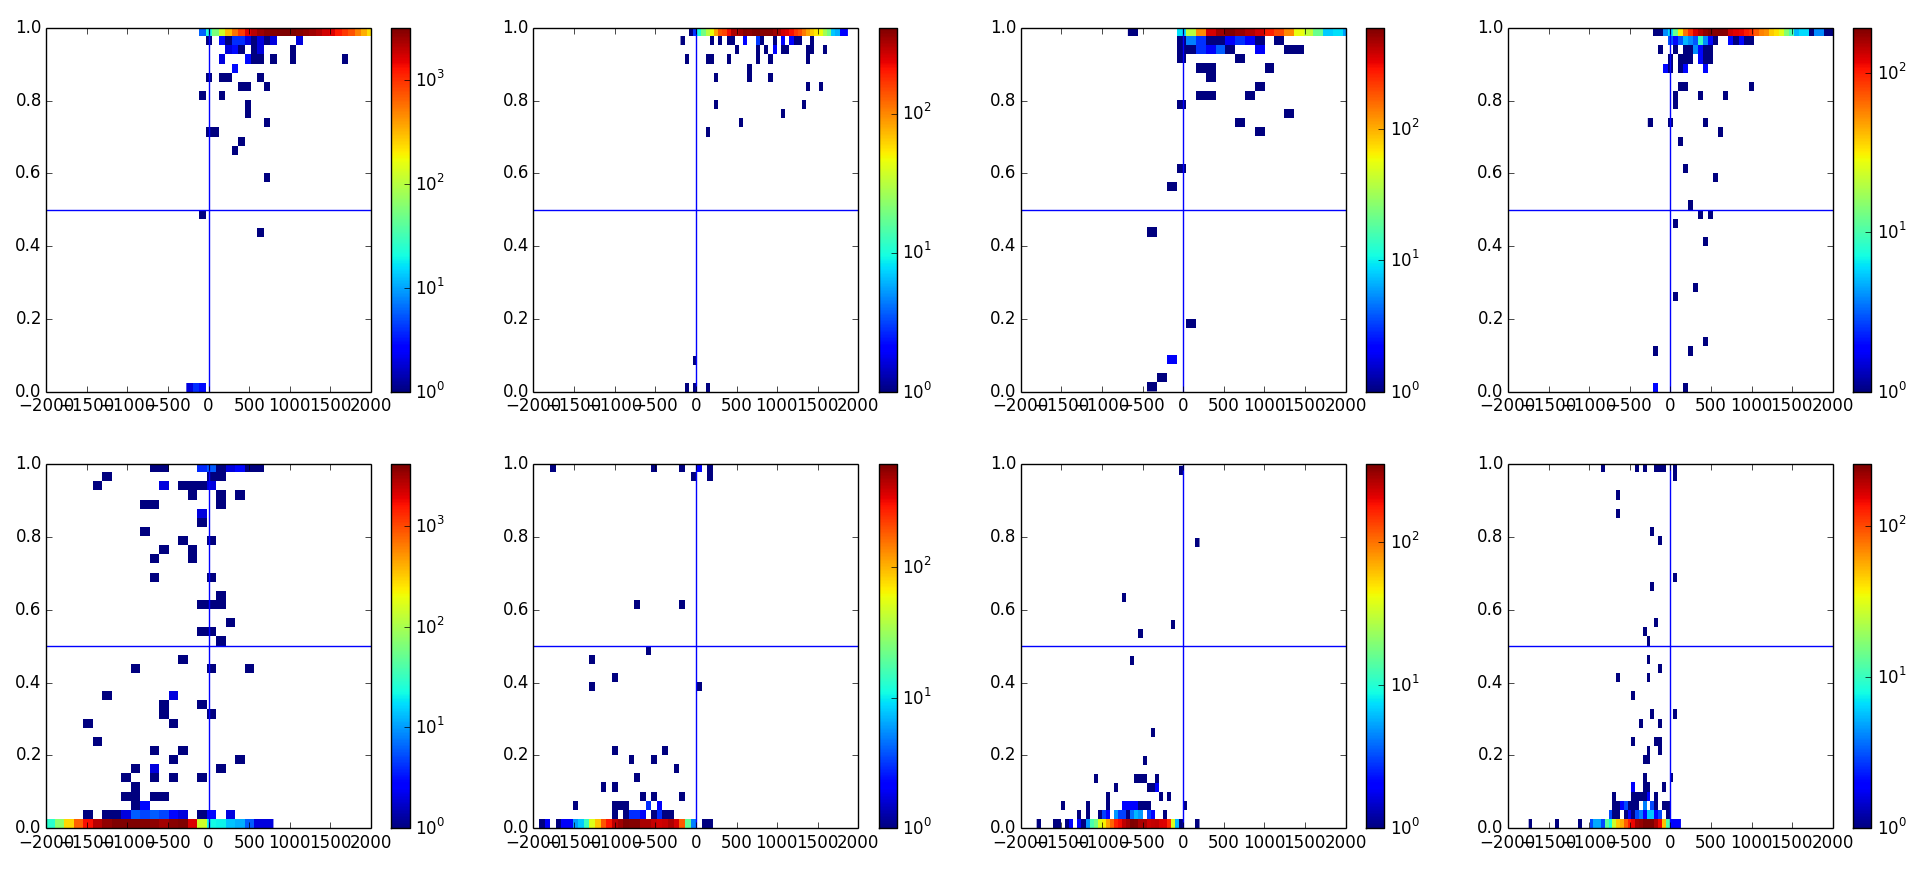
\includegraphics[width=0.48\textwidth]{Phase_Space_Approx.png}
    \caption{Displays of CNN softmax output (y) vs. fiTQun's negative log likelihood (x). Top: electron events, Bottom: muon events. Left to Right: image sets 1, 2, 3, 4.}
    \label{fig:Phase_Space_Approx}
\end{figure}

Investigation of the images where the CNN works but fiTQun fails reveals rings that are greatly distorted, presumably from a bad vertex reconstruction. These distortions do not occur in the case of electrons, as indicated by the strong performance of the fiTQun identification for those particles, which suggests that the CNN recognizes a bad vertex as evidence towards a muon classification by exclusion. To verify that the CNN is not exploiting the failure of fiTQun to artificially inflate its own performance, the analysis was re-conducted using the true vertex position and direction. As expected, the images returned to the normal ring-shapes and the algorithm did not lose performance for muons in the region where fiTQun failed.

\section{Conclusion}

Particle identification in water Cherenkov detectors is done by comparing the Cherenkov profiles of different rings. Since the PMTs act as pixels in an image, and ring shape is a qualitative attribute, it is a natural solution to implement image recognition machine learning methods to classify them. We tested this approach using simulated events in the Super-K detector.

The Super-K standard analysis fitting algorithm is specifically tuned for the problem of electron-muon separation, with complex modelling of Cherenkov light moving and scattering in the detector. The CNN, however, has the advantage that it requires no prior knowledge of Cherenkov physics, and is only tuned in a few generic ways. In fact, all the ring details, besides the initial filters, are learned automatically by the algorithm. The comparable performance of the CNN to the standard particle identification is promising, and these results may be of interest for future analysis.

\section{Acknowledgements}

I would like to thank Stefania Bordoni at CERN and Hirohisa Tanaka at The University of Toronto for their careful supervision throughout the summer, as well as NSERC and Univeristy of Toronto for funding my research. I am also grateful towards The Institute for Particle Physics for giving me the unique opportunity to participate in the CERN Summer Student Program.

%----------------------------------------------------------------------------------------
%	REFERENCE LIST
%----------------------------------------------------------------------------------------

\begin{thebibliography}{99} % Bibliography - this is intentionally simple in this template

\bibitem{cite:SuperK}
\textit{The Super-Kamiokande detector} Nucl. Instrum. Meth. A501 (2003) 418-462

\bibitem{cite:tensorflow}
TensorFlow: \textit{Large-scale machine learning on heterogeneous systems},
2015. Software available from tensorflow.org

\bibitem{cite:fiTQun_poster}
\textit{Improving The T2K Oscillation Analysis With fiTQun}. Poster by Andrew Missert.

t2k.org/docs/poster/076

\bibitem{cite:fiTQun}
Abe K. et al. (the T2K collaboration), \textit{Measurements of Neutrino Oscillation in appearance and disappearance channels by the T2K experiment with $6.6\times 1020$ protons on target}. Phys. Rev. D 91, 072010 (2015). 

\bibitem{cite:CNN}
Notes from the Stanford CS class CS231n: Convolutional Neural Networks for Visual Recognition: 

cs231n.github.io/convolutional-networks/


\end{thebibliography}

%----------------------------------------------------------------------------------------

\end{document}

